\chapter{绪论}
\label{chap:references}

\section{总序}

操作系统的“Page Fault”异常处理例程首先会判断,该数据的虚拟地址是否是该任务的合法地址?根据之前操作系统的设置,答案是“Yes”;然后取出保存在对应页表项中的扇区地址,把存储设备上交换区上对应的虚拟页内容读入到某空闲的物理内存页中;接着更新页表项内容,即把对应的物理页号写入页表项,把页表项中的存在位(Present Bit)置“1”;最后是返回该任务,让该任务重新执行访问数据的指令。这次处理器再次执行这条指令时,TLB还是会没有命中,但由于对应页表项内容合法,所以TLB会缓存该页表项,并完成虚拟地址到物理地址的转换,完成访问数据指令的执行。

相对于内存访问,交换区的扇区访问要慢很多。为了进一步提高系统的执行效率,当操作系统在让存储设备进行I/O访问时,可将当前任务设置为阻塞状态,并切换其他可以运行的任务继续执行。通过这种任务调度方式,可以充分发挥多道程序和分时多任务的整体执行效率

这是2022年暑假参加rCore社区第二阶段的课题, 我接着课题(异步操作系统)继续尝试做的一些工作。课题主要探索利用Rust先天对异步支持的优势来重新设计rCore并尝试为其添加异步的特性。
操作系统设计的意义:
\begin{enumerate}
\item 库操作系统(Library Operating System, 简称 LibOS)是根据某类应用的特殊需求,由某一高级编程语言将原本属于操作系统内核的某些资源管理功能,如文件磁盘 I/O、网络通信等,按照模块化的要求,以库的形式提供给应用程序的特殊操作系统。
它能代替操作系统内核合理地管理和控制所涉及的计算机资源,并将所涉及的计算机
\item 资源直接暴露给应用程序, 让应用程序直接访问底层(虚拟)硬件, 以便应用程序能够高效地运行。特别地,它与应用程序在编译时被链接到一起,形成一个只有单地址空间的二进制文件并工作在应用层,是构建 Unikernel 的一个必不可少的系统组件。
    \begin{itemize}
        \item Linux 作为主流的开源操作系统发展已经走过三十多个年头了,历史的包袱已经略显沉重, 随着物联网的快速袭来, 单片机的开发也日益增多。 Linux Kernel内核中的许多module可能略显多余甚至很多存在功能冗余, 这样不急增加单片机的设计难度还为增加单片机的内存压力。可供定制和模块化良好的库操作系统可以缓解单片机开发中系统的选择匮乏。
    \end{itemize}
\item 异步的另外一种含义是计算机多线程的异步处理。 与同步处理相对, 异步处理不用阻塞当前线程来等待处理完成,而是允许后续操作,直至其它线程将处理完成,并回调通知此线程。
    \begin{itemize}
    \item 异步的需求主要来自任务的并发,而且是发生大量的任务请求。如果同步进行系统响应,那将是一件十分可怕的事情,系统以阻塞的方式对请求进行响应,那可能是一段很长的等待, 尤其可怕的是, CPU存在极大可能是一个空闲的状态。 例如, 存在一个I/O事件, 在请求I/O的控制权之后,CPU将无需为此事件提供服务,那么CPU就会空闲下来,从CPU资源使用的角度看这是十分不可取的,CPU的资源十分宝贵,一定需要让CPU尽可能处于忙的工作环境下。异步,异步的另外一种含义是计算机多线程的异步处理。与同步处理相对,异步处理不用阻塞当前线程来等待处理完成,而是允许后续操作,直至其它线程将处理完成, 并通过全局的唤醒机制回调通知此线程。 从而使得核心资源处于一个忙碌的状态。
    \end{itemize}
\end{enumerate}

Ring\_scheduler\pagescite{tornado0}: 自己的工作是继续tronado-os\pagescite{tornado0}的工作, 实现一个类似shared\_ scheduler的ring\_scheduler,将其接入rCore\pagescite{rcore0}并使得其可以工作在rCore中,并试着将其从内核模块中正交出来,形成一个独立的模块(Crate)。 而异步的设计往往需要底层硬件的支持, 因此需要完成对底层硬件的异步工作,而磁盘的读写被抽象为文件的读写,当硬件的异步完成时,需要对文件系统进行合理的改造使其能完成异步相应的工作需求。ring\_scheduler的接入需要在内核中实例化,提供相应的系统调用。

模块化的设计:预先的设想只是将模块在语言静态编译时就完成所有模块的载入工作,但是得益于Theseus\pagescite{theseus0}的启发,有考虑在所有模块正交完成之后,尝试动态的内核模块的载入,其核心是对每个模块的elf的解析,从而在内核运行时动态载入。上述两者的模块化思路,前者主要依赖于语言的编译时,其实质只是将杂糅在一起的模块通过正交,变成独立且具有层次的的依赖树,模块之间的依赖通过各自之间ABI的调用形成约束;后者主要依赖语言的运行时,是对模块的进一步抽象,因为依赖于语言的运行时,所以需要独立的可以管理模块的内核单元对模块进行树状管理。


\section{动机}

很多程序必须执行大量独立且不需要串行化的任务。例如,数据库服务器可以监听和处理大量的客户端请求。因为这些请求没必要按照某个特定的顺序被处理,他们可以被当作独立的执行单元,原则上他们可以并行地执行。如果系统可以提供子任务并发执行地机制,这些应用程序将会运行得更好。

操作系统中,相对于内存访问,交换区的扇区访问要慢很多。为了进一步提高系统的执行效率,当操作系统在让存储设备进行I/O访问时,可将当前任务设置为阻塞状态,并切换其他可以运行的任务继续执行。通过这种任务调度方式,可以充分发挥多道程序和分时多任务的整体执行效率。


\section{研究背景与意义}

研究目的:异步的提出是为了提高程序在热点事件下的并发性能。

研究意义: 编译器与操作系统进行密切配合,用户态的异步系统调用会同编译器自动生成相应的系统调用请求代码和协程控制块数据结构;只有在第一次系统调用和最后一次系统调用时需要进入内核空间;中间各次的系统调用只进行系统调用结果查询和进程、线程或协程切换。

研究好处: 异步调度下,操作系统应对高并发的任务时,可以获得更好的响应表现,CPU可以一直处在忙碌的状态。无栈的协程,内部的状态转换通过状态机图实现,无需函数主动调用yield,内部也只是状态的转换,无需多余的栈空间开销。

\section{国内外研究现状}

\subsection{国外现状}

\subsubsection{Libaio}

\begin{figure}[htb]
    \figureCapSet
    \centering
    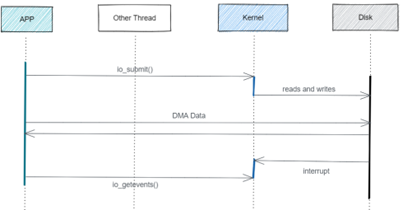
\includegraphics[width=.8\linewidth]{figure/c1/libaio.png}
    \caption{Libaio\pagescite{IoUring1}的工作流}
    \label{figure:c1libaio}
\end{figure}

Libaio的工作流如\autoref{figure:c1libaio}所示, 以read的请求来说, direct IO\pagescite{IoUring1}的模式会把从磁盘上读取的数据直接返回给了用户态的内存空间,不会在内核中缓存,当存在多次重复读取的场景,每次都需要读取磁盘,这样会增加磁盘的压力。


\subsubsection{IO\_URING}

\begin{figure}[htb]
    \figureCapSet
    \centering
    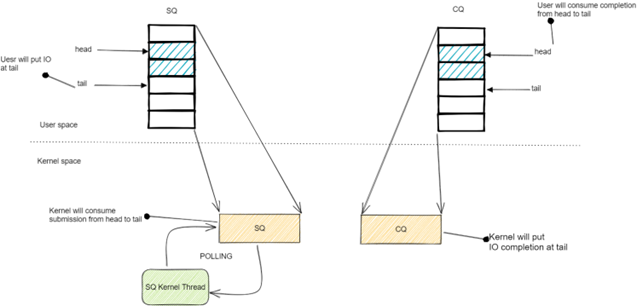
\includegraphics[width=.8\linewidth]{figure/c1/iouring.png}
    \caption{io\_uring\pagescite{IoUring2}的工作流}
    \label{figure:c1iouring}
\end{figure}

io\_uring的工作流如\autoref{figure:c1iouring}所示,io\_uring的基本逻辑与linux-aio\pagescite{IoUring2}是类似的,提供两个接口,一个将I/O请求提交到内核,一个从内核接收完整的事件。但是在设计上是真正的异步。只要设置了合适的参数,在系统调用上下文中只是将请求放入队列,而不会做额外的工作,保证了应用不会被阻塞。io\_uring无需像aio那样使用 poll+read/write来处理sockets,只需要提交一个阻塞式的度,请求完成之后,就会出现在CQ(completion ring)。io\_uring实例有两个环形队列,在内核和用户空间之间共享, 这两个队列都是单生产者、单消费者,提供无锁的接口,内部使用内存屏障同步。

\textbf{io\_uring可以工作在三种模式上}

\begin{enumerate}
\item 中断驱动的默认模式。通过提交相应的I/O请求,然后直接通过CQ状态判断是否完成。
\item 轮询模式,这种模式需要文件系统和块设备支持轮询功能,相比中断驱动模式,这种虽然延迟低,但可能会消耗更多CPU资源。当一个读或写请求提交给轮询上下文之后,应用必须轮询CQ队列,判断请求是否已经完成。
\item 内核轮询模式,这种模式会创建一个内核线程来执行SQ的轮询工作。
\end{enumerate}


使用这种模式的io\_uring实例, 应用无需切到到内核态 就能触发(issue)I/O 操作。通过SQ来提交SQE,以及监控CQ的完成状态,应用无需任何系统调用,就能提交和收割 I/O。


\subsection{国内现状}

\subsubsection{tornado-os的共享调度器}

\begin{figure}[htb]
    \figureCapSet
    \centering
    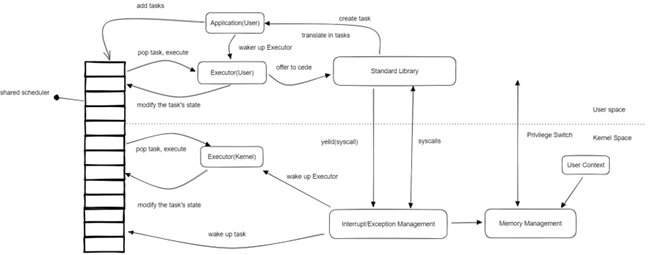
\includegraphics[width=.8\linewidth]{figure/c1/sharedscheduler.png}
    \caption{shared\_scheduler\pagescite{tornado0}的工作流}
    \label{figure:c1sharedscheduler}
\end{figure}

调度器直接将所使用的代码、任务池资源都共享到用户,由用户运行和内核相同的代码,以此与内核以相同的逻辑处理任务池中的任务,从而从共享的任务池中得到下一个任务。

总结一下,基本上,异步系统调用的执行过程应当符合:


\begin{enumerate}
    \item 第一次异步系统调用时
    \begin{itemize}
        \item 用户进程准备系统调用参数、发出系统调用请求;
        \item 内核进程将映射共享内存、发起相应服务协程的异步执行;
        \item 内核进程执行完服务协程后,再响应队列保存返回值,并通过用户态中断通知应用进程;
    \end{itemize}

    \item 第二次异步系统调用时
    \begin {itemize}
        \item 用户进程再请求队列转杯系统调用参数;在共享内存的响应队列中查看一次系统调用的结果;
        \item 内核进程在完成第一个服务协程后,在共享内存的响应队列中保存返回值,主动查询新的系统调用请求,并执行;如果没有新的请求,则让出CPU;
    \end{itemize}
\end{enumerate}

发展:异步的调度的研究应该会是未来网络系统服务的一个方向,随着网络的普及和发展,异步是一种可行的高并发设计思路,是有其研究的价值和意义。



